\documentclass[12pt]{article}
\usepackage{fontspec}
\usepackage{fullpage}
\usepackage{hyperref}
\usepackage{array}
\usepackage{url}
\usepackage{amsmath}
\usepackage{pgfplotstable}
\usepackage{algorithm2e}
\usepackage{multirow}
\usepackage{subcaption}
\usepackage{color}
\usepackage{adjustbox}
\usepackage{tikz}
\usepackage{tikz-dependency}
\usetikzlibrary{shapes,fit,calc,er,positioning,intersections,decorations.shapes,mindmap,trees}
\tikzset{decorate sep/.style 2 args={decorate,decoration={shape backgrounds,shape=circle,
      shape size=#1,shape sep=#2}}}

\newfontfamily\hebfont[Script=Hebrew, Scale=MatchUppercase]{FreeSans}
\newcommand{\heb}[1]{\bgroup\textdir TRT\hebfont #1\egroup}

\title{Universal Semantic Parsing with Neural Networks \\
\heb{ניתוח סמנטי אוניברסלי באמצעות רשתות נוירונים}
}
\date{2018 \heb{דצמבר}}

\begin{document}

\maketitle

\begin{table}[!th]\small
\begin{tabular}{lr>{\bfseries}r}
Daniel Hershcovich & \heb{דניאל הרשקוביץ} & \heb{שם התלמיד:} \\
Prof. Ari Rappoport and Dr. Omri Abend & \heb{פרופ' ארי רפופורט וד"ר עמרי אבנד} & \heb{שמות המדריכים:}
\end{tabular}
\end{table}



\section{Introduction}\label{sec:introduction}

Semantic applications in natural language processing (e.g., machine translation)
require understanding the meaning of text.
Syntactic representations suffer from limitations, since they do not
represent semantic structure directly,
which semantic annotation schemes attempt to do.
In order to represent the full range of semantic structures exhibited by
natural language, three properties should be supported: reentrancy,
representing arguments shared between predicates (Figure~\ref{fig:graduation});
non-terminal nodes for multi-word units (Figure~\ref{fig:home});
and discontinuity of semantic units in the text (Figure~\ref{fig:gave}).
The only semantic annotation scheme that supports the combination of these criteria is UCCA
\cite{abend2013universal}.

\begin{figure}[ht]\small
  \begin{subfigure}{.6\textwidth}
  \parbox{.1\textwidth}{\caption{}\label{fig:graduation}}
  \parbox{.3\textwidth}{
  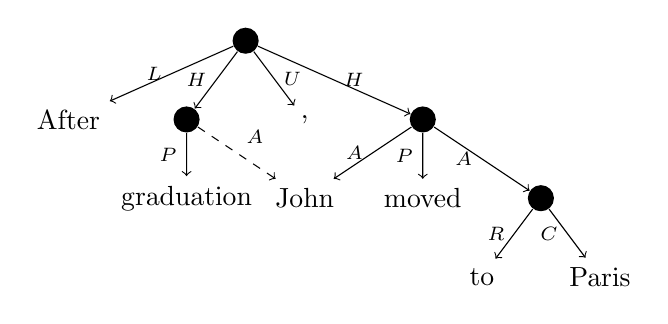
\begin{tikzpicture}[level distance=10mm, ->]
    \node (ROOT) [fill=black, circle] {}
      child {node (After) {After} edge from parent node[left] {\scriptsize $L$}}
      child {node (graduation) [fill=black, circle] {}
      {
        child {node {graduation} edge from parent node[left] {\scriptsize $P$}}
      } edge from parent node[left] {\scriptsize $H$} }
      child {node {,} edge from parent node[right] {\scriptsize $U$}}
      child {node (moved) [fill=black, circle] {}
      {
        child {node (John) {John} edge from parent node[left] {\scriptsize $A$}}
        child {node {moved} edge from parent node[left] {\scriptsize $P$}}
        child {node [fill=black, circle] {}
        {
          child {node {to} edge from parent node[left] {\scriptsize $R$}}
          child {node {Paris} edge from parent node[left] {\scriptsize $C$}}
        } edge from parent node[left] {\scriptsize $A$} }
      } edge from parent node[right] {\scriptsize $H$} }
      ;
    \draw[dashed,->] (graduation) to node [auto] {\scriptsize $A$} (John);
  \end{tikzpicture}
  }
  \end{subfigure}
  \begin{subfigure}{.4\textwidth}
  \parbox{.1\textwidth}{\caption{}\label{fig:home}}
  \parbox{.3\textwidth}{
  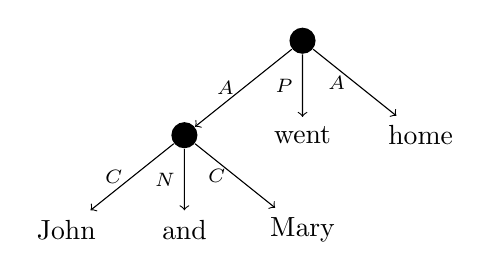
\begin{tikzpicture}[level distance=12mm, ->,
      every node/.append style={midway}]
    \node (ROOT) [fill=black, circle] {}
      child {node [fill=black, circle] {}
      {
        child {node {John} edge from parent node[left] {\scriptsize $C$}}
        child {node {and} edge from parent node[left] {\scriptsize $N$}}
        child {node {Mary} edge from parent node[left] {\scriptsize $C$}}
      } edge from parent node[left] {\scriptsize $A$} }
      child {node {went} edge from parent node[left] {\scriptsize $P$}}
      child {node {home} edge from parent node[left] {\scriptsize $A$}}
      ;
  \end{tikzpicture}
  }
  \end{subfigure}
  \begin{subfigure}{.4\textwidth}
  \parbox{.1\textwidth}{\caption{}\label{fig:gave}}
  \parbox{.3\textwidth}{
  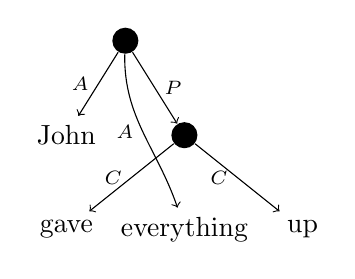
\begin{tikzpicture}[level distance=12mm, ->,
      every node/.append style={midway}]
    \node (ROOT) [fill=black, circle] {}
      child {node {John} edge from parent node[left] {\scriptsize $A$}}
      child {node [fill=black, circle] {}
      {
      	child {node {gave} edge from parent node[left] {\scriptsize $C$}}
      	child {node (everything) {everything} edge from parent[white]}
      	child {node {up} edge from parent node[left] {\scriptsize $C$}}
      } edge from parent node[right] {\scriptsize $P$} }
      ;
    \draw[bend right,->] (ROOT) to[out=-20, in=180] node [left] {\scriptsize $A$} (everything);
  \end{tikzpicture}
  }
  \end{subfigure}
  \begin{subfigure}{.6\textwidth}
  \parbox{.1\textwidth}{\caption{}\label{fig:shower}}
  \parbox{.3\textwidth}{
  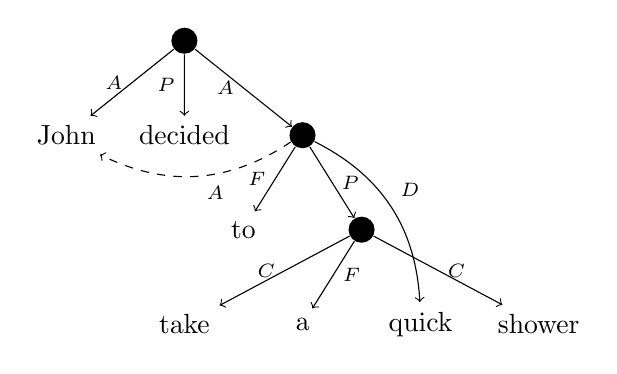
\begin{tikzpicture}[level distance=12mm, ->,
      every node/.append style={midway}]
    \node (ROOT) [fill=black, circle] {}
      child {node (John) {John} edge from parent node[left] {\scriptsize $A$}}
      child {node {decided} edge from parent node[left] {\scriptsize $P$}}
      child {node (totakeaquickshower) [fill=black, circle] {}
      {
        child {node {to} edge from parent node[left] {\scriptsize $F$}}
        child {node [fill=black, circle] {}
        {
          child {node {take} edge from parent node[left] {\scriptsize $C$}}
          child {node {a} edge from parent node[right] {\scriptsize $F$}}
          child {node (quick) {quick} edge from parent[white]}
          child {node {shower} edge from parent node[right] {\scriptsize $C$}}
        } edge from parent node[right] {\scriptsize $P$} }
      } edge from parent node[left] {\scriptsize $A$} }
      ;
    \draw[bend left,dashed,->] (totakeaquickshower) to node [auto] {\scriptsize $A$} (John);
    \draw[bend left,->] (totakeaquickshower) to node [auto] {\scriptsize $D$} (quick);
  \end{tikzpicture}
  }
  \end{subfigure}
  \caption{\label{fig:examples}
    UCCA examples.
    (\subref{fig:graduation}) includes a remote edge (dashed),
    resulting in ``John'' having two parents.
    (\subref{fig:home}) includes a coordination construction (``John and Mary'').
    (\subref{fig:gave}) includes a discontinuous unit (``gave ... up'').
    (\subref{fig:shower}) includes both a remote edge and a discontinuous unit (``take a ... shower'').
    Legend: $P$ -- Process (a Scene's main relation), $A$ -- Participant,
    $L$ -- inter-scene Linker, $H$ -- Parallel Scene, $C$ -- Center, $D$ -- Adverbial,
    $R$ -- Relator, $N$ -- Connector, $U$ -- Punctuation, $F$ -- Function unit.
  }
\end{figure}

Universal Cognitive Conceptual Annotation (UCCA)
is a cross-linguistically applicable semantic representation scheme.
It covers the predicate-argument
structures evoked by predicates of all grammatical categories, the inter-relations between them,
as well as other major linguistic phenomena.
UCCA has demonstrated applicability to multiple languages,
rapid annotation \cite{abend2017uccaapp},
stability in translation \cite{sulem2015conceptual}
and benefit for various applications
\cite{birch2016hume,choshen2018usim,sulem2018samsa,sulem2018simple}.

While semantic representation schemes are different in form and focus,
much of their semantic content is shared \cite{abend2017state}.
Recent work in semantic parsing has targeted
Abstract Meaning Representation \cite{banarescu2013abstract} and
Semantic Dependencies \cite{oepen2016towards}.
Universal Dependencies \cite{nivre2016universal}
is a \textit{syntactic} dependency scheme aiming for cross-lingual consistency,
whose annotation is often similar to the common practice in semantic treebanks
(Figure~\ref{fig:original_example_ud}).

\begin{figure}[th]
  \centering
    \begin{dependency}[text only label, label style={above,font=\tt}, font=\small]
    \begin{deptext}[column sep=.8em,ampersand replacement=\^]
    After \^ graduation \^ , \^ John \^ moved \^ to \^ Paris \\
    \end{deptext}
        \depedge[edge unit distance=1ex]{2}{1}{case}
        \depedge[edge unit distance=1ex]{4}{3}{punct}
        \depedge[edge unit distance=1ex]{5}{4}{nsubj}
        \depedge[edge unit distance=1ex, edge end x offset=-2pt]{2}{5}{obl}
        \depedge[edge unit distance=1ex]{7}{6}{case}
        \deproot[edge unit distance=1.5ex]{5}{root}
        \depedge[edge unit distance=1.5ex]{5}{7}{obl}
    \end{dependency}
\caption{Example UD tree, demonstrating practices common in semantic annotation:
linking content words to content words, and the preference of lexical heads over functional ones.
\label{fig:original_example_ud}}
\end{figure}

My research is concerned with learning to parse UCCA graphs from text, representing its semantics.
I introduce a general graph parser,
and investigate the relationship with other representations to find beneficial commonalities and
differences highlighting the potential utility of semantic parsers for text understanding applications.
The analysis also exposes challenges semantic parsers must address,
and potential sources for improvement.

\section{Goals}\label{sec:goals}

In my research, I pursue the following goals:

\begin{itemize}
  \item Developing techniques for general graph parsing.
    Specifically, devising a method for automatic prediction of UCCA
    structure given plain text.
  \item Investigating and quantifying the relationship between the content
    captured in UCCA and other semantic or syntactic representations.
  \item Taking advantage of the similarities to other schemes,
    to improve UCCA parsing by learning common distinctions.
\end{itemize}


\section{Methods}\label{sec:methods}

\subsection{Transition-Based Parsing}\label{sec:transition_based}

Transition-based parsers \cite{Nivre03anefficient} build trees or graphs
as they scan the text incrementally.
The parse is created by applying a \textit{transition} at each step to the parser state,
defined using a buffer of tokens and nodes to be processed,
a stack of nodes currently being processed,
and a graph of constructed nodes and labeled edges.
A classifier is used at each step to select the next transition based on features
that encode the parser's current state.
During training, an oracle creates training instances for the classifier,
based on the gold-standard annotation.

The transition-based approach has produced some of the best
results in syntactic dependency parsing
\cite{kiperwasser2016simple,andor2016globally}, and has also demonstrated
strong performance in a variety of other semantic and syntactic settings
\cite{maier2015discontinuous,damonte-17}.
Transition-based methods are a natural starting point for UCCA parsing,
as the set of distinctions it represents is similar in spirit to the distinctions
conveyed by dependency schemes.


\subsection{Neural Networks}\label{sec:neural_networks}

Neural networks are powerful machine learning models.
They have yielded state-of-the-art results in many fields,
including natural language processing \cite{goldberg2016primer}.
Inspired by the brain's computation mechanism,
artificial neural networks operate on dense input representations
by a combination of linear and non-linear transformations.

Language data is commonly manifested as sequences
(e.g., sentences are sequences of words).
Recurrent neural networks \cite{elman1990finding} allow representing
arbitrarily sized sequences in a fixed-size vector,
without ignoring the structured properties of the input.
A specific flavor called Long Short Term Memory
(LSTM) is very common as it learns relatively long-term dependencies.
A bidirectional recurrent neural network, such as a BiLSTM,
takes into account both the past and future.


\subsection{Multitask Learning}\label{sec:multitask}

Multitask learning \cite{caruana1998multitask} allows exploiting the overlap between tasks
to effectively extend the training data, 
and has greatly advanced with neural networks and representation learning.
It has been used over the years for NLP tasks with varying degrees of similarity.

Neural multitask learning has mostly been effective in tackling formally similar
tasks \cite{P16-2038},
including
multilingual syntactic dependency parsing \cite{Q16-1031,guo2016exploiting},
as well as multilingual \cite{duong2017multilingual},
and cross-domain semantic parsing \cite{herzig-berant:2017:Short,W17-2607}.

Sharing parameters with a low-level task
has shown great benefit for transition-based syntactic parsing
\cite{bohnet2012transition,Zhang2016StackpropagationIR,constant-nivre:2016:P16-1,more2016joint}.
Recent work has achieved state-of-the-art results in multiple NLP tasks
by jointly learning the tasks forming the NLP standard pipeline using 
a single neural model \cite{collobert2011natural,D17-1206},
thereby avoiding cascading errors, common in pipelines.


\section{Experiments}\label{sec:experiments}

\paragraph{Data.}

Experiments are performed on the English Wikipedia UCCA corpus (Wiki),
the \textit{Twenty Thousand Leagues Under the Sea} UCCA corpora (20K),
annotated in English, French and German;
LDC2017T10 for AMR;
the DM representation from SDP 2016;
and all English, French and German treebanks from UD v2.1.


\paragraph{Evaluation.}
Comparing UCCA structures
$G_p=(V_p,E_p,\ell_p)$ and $G_g=(V_g,E_g,\ell_g)$,
over the same sequence of terminals $W = \{w_1,\ldots,w_n\}$
is done as follows.
For an edge $e=(u,v)$ in either graph, its yield $y(e) \subseteq W$ is the
set of terminals in $W$ that are descendants of $v$.
Define the set of \textit{mutual edges} between $G_p$ and $G_g$:
\[
    M(G_p,G_g) =
    \left\{(e_1,e_2) \in E_p \times E_g \;|\;
    y(e_1) = y(e_2) \wedge \ell_p(e_1)=\ell_g(e_2)\right\}
\]

Labeled precision and recall are defined by dividing $|M(G_p,G_g)|$ by $|E_p|$ and $|E_g|$, respectively,
and F-score by taking their harmonic mean.
Two variants are reported: one where we consider only primary edges,
and another for remote edges


\paragraph{Settings.}

The following settings are explored:
(1) in-domain setting in English, training and testing on Wiki;
(2) out-of-domain setting in English, training on Wiki and testing on 20K;
(3) French in-domain setting, where available training dataset is small,
training and testing on 20K;
(4) German in-domain setting on 20K, with somewhat noisy annotation.
For multitask experiments, we use unlabeled AMR, DM and UD parsing as auxiliary tasks in English,
and unlabeled UD parsing in French and German.

\paragraph{Baselines.}
As no direct comparison with existing parsers is possible,
baselines are bi-lexical dependency graph parsers,
which support reentrancy and discontinuity but not non-terminal nodes;
and \textit{tree approximation}, converting UCCA to (bi-lexical) trees
and evaluating constituency and dependency tree parsers on them.
Baselines are DAGParser \cite{ribeyre-villemontedelaclergerie-seddah:2014:SemEval} and
TurboParser \cite{almeida-martins:2015:SemEval},
two bi-lexical dependency graph parsers;
\textsc{uparse} \cite{maier-lichte:2016:DiscoNLP},
a transition-based constituency parser supporting discontinuous constituents;
and two bi-lexical tree parsers:
MaltParser \cite{nivre2007maltparser},
and the stack LSTM parser \cite{dyer2015transition}.


\paragraph{Results.}

\begin{table}[t]
\centering
\footnotesize
\setlength\tabcolsep{3pt}
\begin{subfigure}{.475\textwidth}
\begin{tabular}{l|lll|lll}
& \multicolumn{3}{c|}{\bf Primary} & \multicolumn{3}{c}{\bf Remote} \\
& \textbf{LP} & \textbf{LR} & \textbf{LF}
& \textbf{LP} & \textbf{LR} & \textbf{LF} \\
\hline
\multicolumn{4}{l|}{\bf English (in-domain)} \\
\multicolumn{4}{l|}{\rule{0pt}{2ex}
Bi-lexical Approximation} \\
DAGParser
& 61.8 & 55.8 & 58.6 & 9.5 & 0.5 & 1 \\
TurboParser
& 57.7 & 46 & 51.2 & 77.8 & 1.8 & 3.7 \\
\hline
\multicolumn{4}{l|}{\rule{0pt}{2ex}
Tree Approximation} \\
\textsc{uparse}
& 60.9 & 61.2 & 61.1 & -- & -- & -- \\
\hline
\multicolumn{4}{l|}{\rule{0pt}{2ex}
Bi-lexical Tree Approximation} \\
MaltParser
& 62.8 & 57.7 & 60.2 & -- & -- & -- \\
LSTM Parser
& 73.2 & 66.9 & 69.9 & -- & -- & -- \\
\hline
Single
& 74.4 & 72.9 & 73.6 & 53 & 50 & 51.5 \\
Multitask &&& \\
AMR
& 74.7 & 72.8 & 73.7 & 48.7 & 51.1 & 49.9 \\
DM
& 75.7 & 73.9 & 74.8 & 54.9 & 53 & \textbf{53.9} \\
UD
& 75 & 73.2 & 74.1 & 49 & 52.7 & 50.8 \\
AMR + DM
& 75.6 & 73.9 & 74.7 & 49.9 & 53 & 51.4 \\
AMR + UD
& 74.9 & 72.7 & 73.8 & 47.1 & 50 & 48.5 \\
DM + UD
& 75.9 & 73.9 & \textbf{74.9} & 48 & 54.8 & 51.2 \\
All
& 75.6 & 73.1 & 74.4 & 50.9 & 53.2 & 52
\end{tabular}\label{tab:id_results}
\vspace{24.5mm}
\end{subfigure}
\hfill
\begin{subfigure}[t]{.475\textwidth}
\begin{tabular}{l|lll|lll}
& \multicolumn{3}{c|}{\bf Primary} & \multicolumn{3}{c}{\bf Remote} \\
& \textbf{LP} & \textbf{LR} & \textbf{LF}
& \textbf{LP} & \textbf{LR} & \textbf{LF} \\
\hline
\multicolumn{4}{l|}{\bf English (out-of-domain)} \\
\multicolumn{4}{l|}{\rule{0pt}{2ex}
Bi-lexical Approximation} \\
DAGParser
& 56.4 & 50.6 & 53.4 & -- & 0 & 0 \\
TurboParser
& 50.3 & 37.7 & 43.1 & 100 & 0.4 & 0.8 \\
\hline
\multicolumn{4}{l|}{\rule{0pt}{2ex}
Tree Approximation} \\
\textsc{uparse}
& 52.7 & 52.8 & 52.8 & -- & -- & -- \\
\hline
\multicolumn{4}{l|}{\rule{0pt}{2ex}
Bi-lexical Tree Approximation} \\
MaltParser
& 57.8 & 53 & 55.3 & -- & -- & -- \\
LSTM Parser
& 66.1 & 61.1 & 63.5 & -- & -- & -- \\
\hline
Single
& 69 & 69 & 69 & 41.2 & 19.8 & 26.7 \\
Multitask &&& \\
AMR
& 69.5 & 69.5 & 69.5 & 42.9 & 20.2 & 27.5 \\
DM
& 70.7 & 70.7 & 70.7 & 42.7 & 18.6 & 25.9 \\
UD
& 69.6 & 69.8 & 69.7 & 41.4 & 22 & 28.7 \\
AMR + DM
& 70.7 & 70.2 & 70.5 & 45.8 & 19.4 & 27.3 \\
AMR + UD
& 70.2 & 69.9 & 70 & 45.1 & 21.8 & 29.4 \\
DM + UD
& 70.8 & 70.3 & 70.6 & 41.6 & 21.6 & 28.4 \\
All
& 71.2 & 70.9 & \textbf{71} & 45.1 & 22 & \textbf{29.6} \\
\hline
\multicolumn{4}{l|}{\bf French (in-domain)} & \\
Single & 68.2 & 67 & 67.6 & 26 & \enskip 9.4 & 13.9 \\
UD & 70.3 & 70 & \textbf{70.1} & 43.8 & 13.2 & 20.3 \\
\hline
\multicolumn{4}{l|}{\bf German (in-domain)} & \\
Single & 73.3 & 71.7 & 72.5 & 57.1 & 17.7 & 27.1 \\
UD & 73.7 & 72.6 & \textbf{73.2} & 61.8 & 24.9 & \textbf{35.5}
\end{tabular}\label{tab:ood_results}
\end{subfigure}
\caption{
Labeled precision, recall and F-score (in~\%)
on Wiki (left) and 20K (right).
}\label{tab:results}
\end{table}

Table~\ref{tab:results} presents the results.
The stack LSTM parser obtains the highest primary F-score
among the baseline parsers, with a considerable margin. However,
tree approximation parsers are unable to recover any remote edges,
removed in the conversion.
The bi-lexical DAG parsers are quite limited in this respect as well.
The direct UCCA parser, based on BiLSTMs, outperforms all baselines.
Multitask further improves the primary F-score over the single task parser,
but using all auxiliary tasks contributes less than just DM and UD.
For 20K, improvements from using multitask are even more marked. 
Moreover, the improvement is largely additive.
The best multitask models are significantly better than single-task models,
demonstrating that even a small training set for the main task may suffice,
given enough auxiliary training data (as in French).

\paragraph{Discussion.}

Task similarity is an important factor in multitask learning
\cite{E17-2026,E17-1005}.
Empirical comparison with UD reveals that most content differences between it and UCCA are due to:
  \begin{enumerate}
      \item UCCA's distinction of Scene-evoking words and phrases, absent in UD.
      \item UCCA's distinction between primary relations, secondary relations
        and Participants, in contrast to UD's core/non-core distinction.
      \item Different treatment of multi-word expressions (MWEs),
        where UCCA has a stronger tendency to explicitly mark them.
      \item UCCA's conflation of several syntactic realizations of inter-clause linkage,
        and disambiguation of other cases that UD treats similarly.
   \end{enumerate}

  The differences between the schemes are substantial, and suggest that
  UCCA parsing in particular and semantic parsing in general are likely to benefit
  downstream text understanding applications.
  For example, only 73\% of arguments are shared between UCCA and UD,
  i.e., many semantic participants cannot be recovered from UD.

\section{Significance}\label{sec:significance}


Despite the recent diversity of semantic parsing work,
the effectiveness of different approaches for
structurally and semantically different schemes is not well-understood
\cite{kuhlmann2016towards}.
Our contribution to this literature is a general parser
that supports multiple parents, discontinuous units and non-terminal nodes.

A parser for UCCA will enable using the framework for new tasks,
in addition to existing applications such as machine translation
evaluation \cite{birch2016hume}.
We believe UCCA's merits in providing a cross-linguistically applicable,
broad-coverage annotation will support ongoing efforts to incorporate deeper
semantic structures into various applications,
such as sentence simplification \cite{narayan2014hybrid} and summarization \cite{liu2015toward}.


We demonstrate that semantic parsers can leverage a range of 
semantically and syntactically annotated data, to improve their performance.
Our experiments show that MTL improves UCCA parsing,
using AMR, DM and UD parsing as auxiliaries.
We propose a unified DAG representation, 
construct protocols for converting these schemes into the unified format,
and generalize a transition-based DAG parser to support all these tasks,
allowing it to be jointly trained on them.

While we focus on UCCA in this work, our parser is capable of parsing any
scheme that can be represented in the unified DAG format,
and preliminary results on AMR, DM and UD are promising.

UCCA may have a substantial impact on various semantic NLP tasks. For example,
for machine translation, many approaches currently rely on syntactic parsing as
a component, assuming that syntactic structures in one languages tend to be
translated to the same structures in another language. However, UCCA is more
stable than syntactic annotation cross-linguistically, when looking at
translated sentences\cite{sulem2014thesis}. Indeed, UCCA directly represents
the meaning of the text, which is invariant to translation (by the definition
of the translation task), whereas syntax is only a proxy that varies between
languages.

Recent work in neural networks-based machine translation provide some sort of
an intermediate encoding in the form of distributed representation that can be
encoded from the source language and then decoded into the target
language\cite{zou2013bilingual}, or using memory and treating the text as a
sequence to be converted to another sequence\cite{sutskever2014sequence}.
However, the encoding is based just on averaging across words in the source
sentence, on a flat sequence representation, or at best on a syntactic
representation. A semantic representation like a UCCA graph would perhaps be a
better candidate for the structure by which the encoding and decoding is
performed.

Perhaps just as critical as the successful prediction of UCCA structure, if not
even more critical for the NLP community, is the distributed representation
created when forming phrases using this structure. Current methods in NLP form
multi-word representation based on averaging across words or on syntax, which
may be sub-optimal in representing the true meaning of text. Using a more
semantically faithful way to compose words, such as UCCA, may be a key factor
in enabling computers to understand natural language.



\section{Challenges}\label{sec:challenges}

\paragraph{Dataset size.}
Models with a large number of parameters typically require training on very
large datasets, and the number of parameters in a deep learning model usually
scales linearly with the number of layers and quadratically with the size of
the representation, along with other factors that may require more parameters.
Since the UCCA dataset is small in relation to other datasets (such as the Penn
Treebank), training deep learning models on it may pose a challenge.
However, as the experimental results show, the neural network-based LSTM parser
already reaches very high scores on the UCCA task.
Furthermore, the dataset can be enlarged and extended to more languages by further
labeling efforts.


\paragraph{Scheme coarseness.}
The UCCA framework was developed with the foundational layer first, including
relation types that are mainly relevant for syntax. This layer gives only a
coarse annotation: for examples, it labels processes or states and their
participants, but not the role of each participant. The intention is to
gradually refine the annotation to include more fine-grained relation types,
starting with the simplest distinctions. It is possible that learning
the foundational layer alone is easier than learning a more
refined annotation, which would require deeper semantic understanding.
This remains to be investigated when refinements are introduced.

The coarseness of the foundational layer may mean it is not
sufficiently informative for assisting in semantic tasks, because they may
depend on more refined distinctions. However, for many tasks it should be
enough already, as the semantic distinctions that are apparent in syntax are
already covered in the scheme.

\section{Required Resources}\label{sec:resources}

The resources currently used in my research are the
UCCA Wikipedia corpus and the
UCCA \textit{Twenty Thousand Leagues Under the Sea} English-French parallel corpus.
In order to demonstrate the universality of the UCCA scheme and the advantages of its general structure,
it needs to be applied to more languages and domains.
Specifically, as discontinuous constructions are especially abundant in languages such as German
\cite{maier2015discontinuous}, a German corpus annotated with UCCA will be a valuable resource for evaluating
parsers for BSS.
The universality should be assessed further by experimenting with languages even more different than English,
such as Chinese. This will require constructing annotated corpora with native speakers of these languages.


\section{Work Plan}\label{sec:plan}

I intend to further explore conversion-based parsing approaches,
including different target representations and more sophisticated conversion
procedures \cite{kong-15},
to shed light on the commonalities and differences between representations,
suggesting ways to design better semantic representations.
I believe that UCCA's merits in providing a cross-linguistically applicable,
broad-coverage annotation will support ongoing efforts to incorporate deeper
semantic structures into a variety of applications, such as machine translation
\cite{jones2012semantics} and summarization \cite{liu2015toward}.

In the coming year, I will focus my research on improving the different parsing approaches
(\S\ref{sec:improving_conversions} and \S\ref{sec:improving_bsp}).
In the following year, I intend to continue my research by demonstrating the effectiveness
of the parser when applied to semantic tasks (\S\ref{sec:semantic_tasks}).


\subsection{Improving the conversion procedure}\label{sec:improving_conversions}
Several decisions have to be made in the conversion between dependency and
constituency annotation.
Currently, I handle these decisions by heuristics, but a more
sophisticated way can be devised \cite{fernandez2015parsing}.
These will be reflected by higher upper bounds, and a more realistic evaluation
of the performance of existing technology on the UCCA parsing task.
Several of these decisions can be deferred to a machine learning solution,
to improve their accuracy:

\paragraph{Head selection in constituency-to-dependency conversion.}
In the conversion from constituency to dependency, a head terminal has to be
selected for each node. One of the advantages of UCCA is the fact that it is not bound
to select a head for a unit when the selection would be arbitrary, whereas dependency
annotations are. However, some of the head selection rules are justified, and a
better strategy here would improve the accuracy of converted dependency graphs.
I will investigate methods for more informed head selection.

\paragraph{Edge labeling in dependency-to-constituency conversion.}
When converting from dependency to constituency, labels for the
added edges have to be determined, since the intermediate non-terminal nodes are absent
from the dependency graph. I will improve the labeling algorithm to
increase the accuracy of restored UCCA graphs after conversion.

\paragraph{Attachment position in dependency-to-constituency conversion.}
Restored non-terminals are always assumed to be high-attaching, even though
in some cases this decision is incorrect.
I will modify the algorithm to select the correct attachment position for the introduced nodes.

\paragraph{Restoring unary nodes in dependency-to-constituency conversion.}
Unary nodes are missing from the restored graphs, even though they exist in the
original annotation. In order for the conversion to be accurate, these nodes have to
be restored.
I will apply machine-learning methods \cite{fernandez2015parsing} to restore these unary nodes.

\subsection{Improving the direct parser}\label{sec:improving_bsp}
\textsc{bsp} reaches promising results, but it is very basic in terms of the
techniques used in it: for this reason, it currently reaches lower scores than parsers
with a simpler transition system but better classification and inference techniques.

\paragraph{Beam search.}
Using beam search rather than greedy inference should improve the parsing
scores significantly, as it does for many parsers, as it enables maintaining multiple candidates
for the best action sequence, correcting for mistakes made early in the parse when
not enough of the input was seen to make an accurate prediction.
I will implement beam search in \textsc{bsp} and evaluate its contribution to the parsing accuracy.

\paragraph{Embedding features.}
The parser currently uses hand-crafted features, which may not be the best
representation for the classifier to be able to accurately predict the correct action
at each step. Although feature ablation experiments showed that each of the feature
sets has a positive contribution, they can probably be improved to reach higher scores.
As an example, using embeddings for features rather than binary
indicators will enable sharing information across similar tokens and more efficient
representation \cite{chen2014fast},
and a BiLSTM-based distributed representation may be an even better representation
\cite{kiperwasser2016simple}.
I will try both of these approaches.

\paragraph{Neural network classifier.}
Linear classifiers trained with the perceptron algorithm have been used in
dependency parsing extensively, but different models have recently yielded improved
results.
As the experiment with the LSTM parser shows, implementing a parser
based on recurrent neural networks should also give a significant improvement to
parsing scores.
Even neural network models with input from a fixed window (rather than a full recurrent
history) achieve state-of-the-art scores in dependency parsing
\cite{chen2014fast,andor2016globally}, and should boost the performance of \textsc{bsp}.
I will apply different neural architectures to \textsc{bsp} and compare them.

\subsection{Applying the parser to semantic tasks}\label{sec:semantic_tasks}
In order to evaluate the contribution of UCCA and \textsc{bsp} to semantic tasks,
I intend to perform experiments using it to calculate distributed representations for
phrases and sentences, and to derive various features whose impact can be assessed quantitatively.

\paragraph{Sentiment analysis.}
Earlier work on sentiment analysis either ignores the text structure (e.g. using a bag-of-words approach), or
combines distributed representation along a syntactic structure \cite{socher2013recursive}.
I will use the automatic methods for UCCA parsing to build sentiment classifiers that calculate semantic composition
using a semantic structure, and asses whether the resulting representation contributes to the accuracy of the
classifiers as compared to syntactic representation.
Distributed representation of phrases and sentences is useful for a variety of semantic tasks,
but sentiment analysis is a relatively common and important one where compositionality plays a major role:
for example, negation words and intensifiers modify the value of composed phrases, and correctly identifying
their arguments is crucial.


\paragraph{Machine translation.}
Syntax-based machine translation works by either giving syntactically-plausible target sentences higher scores,
or by using syntactic transduction grammars to go through an intermediate syntactic representation between
the source language and the target language \cite{nadejde2013edinburgh}.
Despite their theoretical soundness, syntactic machine translation methods still lag behind simpler methods
such as phrase-based machine translation.
I will investigate ways in which UCCA can replace syntactic structures in these techniques, and perhaps
yield better models.
The advantage of UCCA as compared to syntactic annotation schemes for machine translation is apparent,
as translation tends to preserve semantic structure more than syntactic structure \cite{sulem2015conceptual}.
Using UCCA as an intermediate representation is thus likely to achieve translated sentences that are more
semantically similar to the source.

%\paragraph{Automatic summarization.}
%Similarly to machine translation, meaning representation can be used for abstractive summarization:
%the text is first converted to an abstract representation, and then a summary is generated from the abstract
%representation. Previous work used AMR \cite{banarescu2013abstract} for this approach \cite{liu2015toward}.
%I intend to use UCCA and quantify the contribution of the fact that the scheme is grounded on the words of the
%text to the accuracy of both encoding into an abstract representation and decoding it to generate the summary.


\bibliography{references}
\bibliographystyle{plain}
\end{document}
